\documentclass[12pt]{report}

\usepackage[a4paper]{geometry}
%\geometry{left=2.5cm,right=2.5cm,top=2.5cm,bottom=2.5cm, a4paper}
\usepackage[utf8]{inputenc}
\usepackage{amsmath}
\usepackage{amsthm}
\usepackage{amssymb}
\usepackage{ulem}
\usepackage{graphicx}
\usepackage{caption}
\graphicspath{}
\usepackage[document]{ragged2e}
\usepackage{setspace}
\usepackage{tabularx}
\usepackage[slovene]{babel}
\usepackage{textcomp, gensymb}
\usepackage{siunitx}
\usepackage{pdfrender,xcolor}
\usepackage{hyperref}
\usepackage{xurl}
\usepackage{float}
\usepackage{titlesec}

\newfloat{slika}{htbp}{loc}
\floatname{slika}{Slika}

\newfloat{tabela}{htbp}{loc}
\floatname{tabela}{Tabela}

\title{
  
\includegraphics[width=0.4\textwidth]{fmf_logo}\\
  {\small Oddelek za fiziko} \\
  {Toplotna prevodnost}\\
  {\small Poročilo pri fizikalnem praktikumu III}\\

}
\date{}
\author{ avtor: Kristofer Č. Povšič \\[5 cm]
 \small  Asistentka: Jelena Vesić
}


\titleformat{\chapter}[hang]{\Huge\bfseries}{\thechapter{. }}{0pt}{\Huge\bfseries}

\setlength\parindent{0pt}

\begin{document}

\setcounter{page}{2}

\maketitle

\chapter*{Uvod}

V telesu, ki ima neenakomerno temperaturo, toplota prehaja z delov z višjo na dele z nižjo temperaturo.Toplotni tok ima enačbo

\begin{equation}
  \vec{j}= - \lambda \text{grad}T
\end{equation}

$\lambda$ je koeficient toplotne prevodnosti in se razlikuje za vsako snov. Kovine oz. el. prevodniki so tudi dobri toplotni prevodniki, el. izolatorji pa slabo. 

Toplotna prevodnost in el. prevodnost sta v kovinah povezani preko Wiederman-Franzovega zakona. 

Za meritev toplotne prevodnosti v merjencu vzpostavimo stacionarno ravnovesje. Meritve olajša tudi preprosta geometrijska oblika: palica za dobre prevodnike in plošča/valj pa za slabe. Toplotni tok plošče/palice je: 

\begin{equation}
  j = - \lambda \frac{\Delta T}{l}
\end{equation}

kjer je $\Delta T$ razlika temperatur, $l$ pa dolžina palice. 

V telesu se temperatura $T(\vec{r})$ spreminja z

\begin{equation}
  \frac{\partial T}{\partial t} = D \nabla^2T
\end{equation}

kjer je $D = \frac{\lambda}{\rho c_p}$  toplotna difuzija, $\rho$ gostota, $c_p$ specifična toplotna kapaciteta pri konstantnem tlaku. 

\chapter*{Naloga}

\begin{enumerate}
  \item Umeri termočlen - izmeri zvezo med temperaturo razliko in napetostjo na termočlenu. 
  \item Izmeri koeficiente toplotne prevodnosti 
\end{enumerate}

\begingroup
\let\clearpage\relax

\chapter*{Potrebščine}
\begin{itemize}
  \item merjenec - valj iz neznane kovine 
  \item posoda za hlajenje z vodo, 2 kovinski izolirni posodi 
  \item ledomat in kuhalnik za vodo
  \item električni kuhalnik za olje, variak, električni grelec za vodo - bojler 
  \item termočlen baker-konstantan, termonapetosti $43\mu VK^{-1}$
  \item mikrovoltmeter 
  \item dva digitalna termometra z določeno napako
\end{itemize}

\chapter*{Navodilo}
Najprej umerimo termočlen. Temperaturno razliko med posodo z ledom in posodo z vročo vodo merimo z termometrom. Pri vsaki temperaturi zabeležimo napetosti in narišemo regresivno premico. Temperaturni koeficient termočlena je enak naklonu krivulje. 

Termočlen nato vtaknemo v luknjici na valjastem prevodniku. Pri različnih močeh grelca zapišemo napetost na termočlenu in regresiramo premico. 
\endgroup


\chapter*{Obdelava podatkov}

Za prvi del meritev sem dobil sledeče podatke: 


\begin{tabela}[H]
  \centering
  \[
  \begin{array}{|c|c|} \hline
    \Delta T [K] & U[mV] \\ \hline
    88.60 &    3.70\\
    84.90 &    3.57\\
    80.90 &    3.40\\
    72.90 &    3.07\\
    68.90 &    2.90\\
    65.00 &    2.73\\
    58.30 &    2.47\\
    54.40 &    2.30\\
    49.50 &    2.01\\
    42.60 &    1.73\\
    40.50 &    1.64 \\ \hline
 \end{array}
 \]
\end{tabela}


Izrišem sledeč graf: 

\begin{slika}[H]
  \centering
  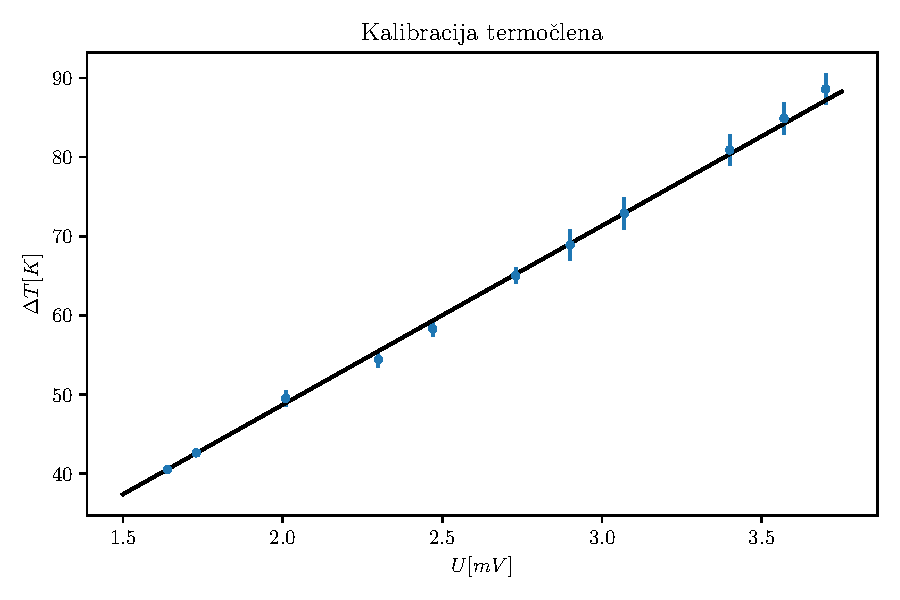
\includegraphics{kalibracija}
  \caption{\small $\Delta T$ med posodo z ledom in posodo z vročo vodo in pri njih izmerjene napetosti na termočlenu. }
\end{slika}

Koeficient premice je 

\[ k = (22.6 \pm 0.4) \frac{K}{V}\]


Za drugi del izmerim sledeče podatke: 


\begin{tabela}[H]
  \centering
  \[
  \begin{array}{|c|c|}\hline
    P[W] & U[mV] \\ \hline
    30.5 &   228.0\\
    35.0 &   275.0\\
    40.0 &   306.0\\
    44.7 &   348.0\\
    50.0 &   378.0\\
    55.9 &   409.0\\
    60.5 &   449.0 \\ \hline
\end{array}
\]
\end{tabela}

Valjast prevodnik ima polmer $R = (4.46 \pm 0.1)cm$ in luknjici sta oddaljeni $l = (5.6 \pm 0.1)cm$. 

Izrišem sledeč graf: 

\begin{slika}[H]
  \centering
  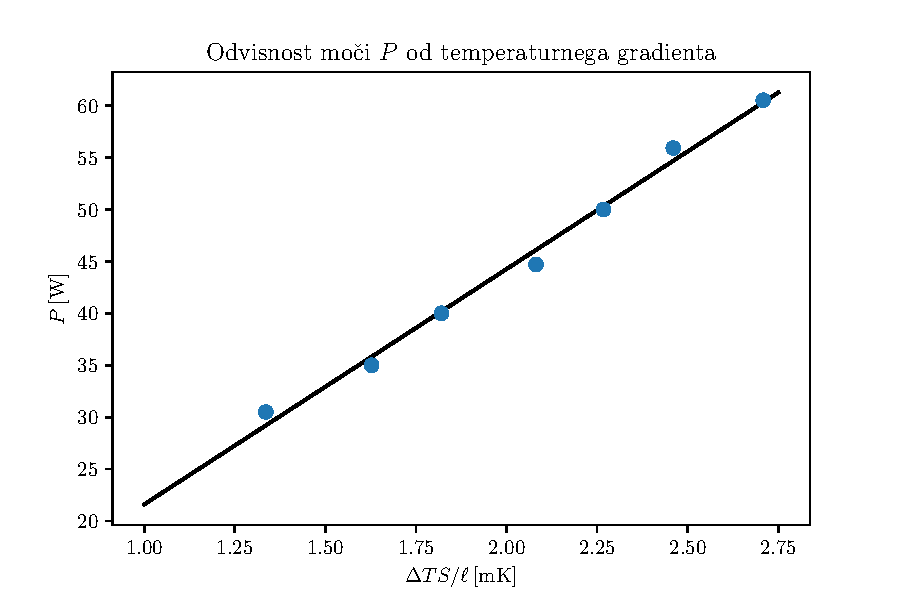
\includegraphics{lambda-fit}
  \caption{\small Moč v odvisnost od napetosti.}
\end{slika}

Regresivna premica ima naklon 

\[k = (226 \pm 9)W/mK\]

kar je tudi koeficient toplotne prevodnosti. 

\end{document}